\documentclass{standalone}
\usepackage{tikz}
\usepackage{ctex,siunitx}
\usepackage{tkz-euclide}
\usepackage{amsmath}
\usetikzlibrary{patterns, calc}
\usetikzlibrary {decorations.pathmorphing, decorations.pathreplacing, decorations.shapes,}
\begin{document}
\small
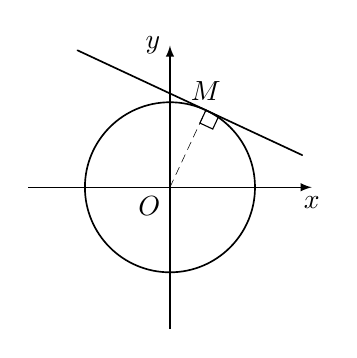
\begin{tikzpicture}[>=latex,scale=0.9]
  \draw[thin,->](-2,0)--(2,0)node[below]{$x$};
  \draw[thin,->](0,-2)--(0,2)node[left]{$y$};
  \tkzDefPoints{0/0/O}
  \tkzDefShiftPoint[O](65:1.2){M}
  \tkzDefShiftPoint[M](-25:1.0){M'}
  \draw[semithick](O)circle(1.2);
  \tkzDrawLine[semithick,add=2 and 0.5](M,M')
  \tkzDrawSegments[densely dashed](O,M)
  \tkzMarkRightAngle[size=0.2](O,M,M')
  % \tkzDrawPoints[fill=black](C)
  % \draw(C)--++(45:1.2)node[midway,above]{$r$};
  % \node at ([shift=(45:1.2)]C)[above right]{$M$};
  \tkzLabelPoints[below left](O)
  \tkzLabelPoints[above](M)
\end{tikzpicture}
\end{document}